\documentclass[tikz, svgnames]{standalone}

\usepackage{mathtools}
\usetikzlibrary{decorations.markings}

\def\V{10}
\def\p{7}

\tikzset{decoration={markings, mark=at position 0.5 with {\arrow{stealth}}}}

\begin{document}
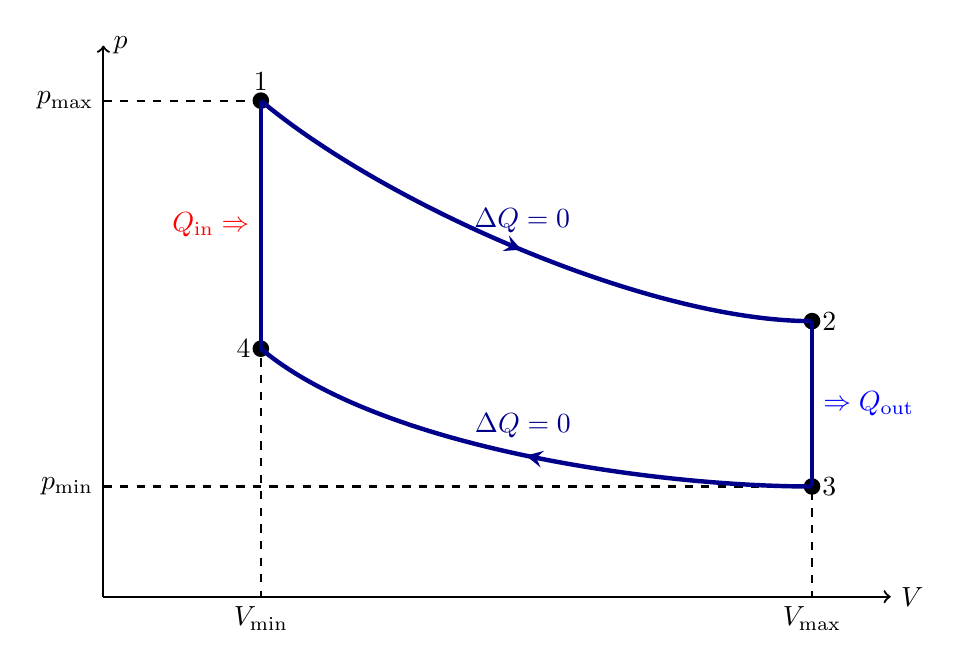
\begin{tikzpicture}[thick]
  \draw[->] (0, 0) -- (0, \p) node[right] {$p$};
  \draw[->] (0, 0) -- (\V, 0) node[right] {$V$};

  \draw[dashed] (0, 0.9*\p) node[left] {$p_\text{max}$} -| (0.2*\V, 0) node[below] {$V_\text{min}$};

  \draw[dashed] (0, 0.2*\p) node[left] {$p_\text{min}$} -| (0.9*\V, 0) node[below] {$V_\text{max}$};

  \coordinate[label=above:1] (a) at (0.2*\V, 0.9*\p);
  \coordinate[label=right:2] (b) at (0.9*\V, 0.5*\p);
  \coordinate[label=right:3] (c) at (0.9*\V, 0.2*\p);
  \coordinate[label=left:4] (d) at (0.2*\V, 0.45*\p);

  \foreach \point in {a, b, c, d}
  \fill (\point) circle (3pt);

  \draw[ultra thick, DarkBlue] (a) edge[out=-40, in=180, looseness=0.7, postaction={decorate}]
  node[midway, above=2px] {$\Delta Q = 0$} (b) (b) -- (c)
  node[midway, right, blue] {$\Rightarrow Q_\text{out}$} (c)
  edge[out=180, in=-40, looseness=0.7, postaction={decorate}]
  node[midway, above=2px] {$\Delta Q = 0$} (d) (d) -- (a)
  node[midway, left, red] {$Q_\text{in} \Rightarrow$};

\end{tikzpicture}
\end{document}
